% !Mode:: "TeX:UTF-8"
%!TEX program  = xelatex

\documentclass{cumcmthesis}
%\documentclass[withoutpreface,bwprint]{cumcmthesis} %去掉封面与编号页

\usepackage{url}
\title{基于非稳态导热的高温作业专用服装设计}
\tihao{A}
\baominghao{4321}
\schoolname{XX大学}
\membera{小米}
\memberb{向左}
\memberc{哈哈}
\supervisor{老师}
\yearinput{2017}
\monthinput{08}
\dayinput{22}

\begin{document}

 \maketitle
 \begin{abstract}
cumcmthesis 是为全国大学生数学建模竞赛编写的\LaTeX{}模板, 旨在让大家专注于 论文的内容写作, 而不用花费过多精力在格式的定制和调整上. 本手册是相应的参考, 其 中提供了一些环境和命令可以让模板的使用更为方便. 同时需要注意, 使用者需要有一 定的 \LaTeX{} 的使用经验, 至少要会使用常用宏包的一些功能, 比如参考文献,数学公式,图片使用,列表环境等等. 例子文件参看 example.pdf.

另外, 欢迎大家购买我们是视频教程,点击\href{https://item.taobao.com/item.htm?spm=a1z10.1-c.w4004-3473795048.4.ThFQCG&id=43823508044}{\fbox{这里}}。

欢迎大家到QQ群里沟通交流:91940767.

\keywords{克兰克-尼科尔森方法\quad  曲线拟合\quad   非线性优化模型\quad  受力分析}
\end{abstract}

%目录
\tableofcontents

\section{问题重述}

    \subsection{问题背景}
    服装作为人与环境之间的中间体,其不同的功能特性保证人类能从事相应的生产
    活动。不同环境下的服装性能被愈加重视。其中高温作业专用服装的设计被高度
    重视,国内外在该方面开展广泛的研究。因此建立高温作业专用服装的数学模型,
    并由此根据环境对皮肤温度进行合理评估,进而通过温度要求对服装厚度和材料
    选取实现最优设计显得尤为重要。

    \subsection{问题重述}
      高温环境下工作时人们需要穿着专用服装以避免灼伤。专用服装通常由三层织物材
    料构成,I层与外界环境接触,III层与皮肤之间还存在空隙,空隙记为IV层。
      为设计专用服装,将体内温度控制在37ºC的假人放置在实验室的高温环境中,测量
    假人皮肤外侧的温度。为了降低研发成本、缩短研发周期,请你们利用数学模型来确
    定假人皮肤外侧的温度变化情况,并解决以下问题:
    (1) 专用服装材料的某些参数值由附件1给出,对环境温度为75ºC、II层厚度为6 mm、
        IV层厚度为5 mm、工作时间为90分钟的情形开展实验,测量得到假人皮肤外侧的
        温度(见附件2)。建立数学模型,计算温度分布,并生成温度分布的Excel文件
        (文件名为problem1.xlsx)。
    (2) 当环境温度为65ºC、IV层的厚度为5.5 mm时,确定II层的最优厚度,确保工作60
        分钟时,假人皮肤外侧温度不超过47ºC,且超过44ºC的时间不超过5分钟。
    (3) 当环境温度为80 时,确定II层和IV层的最优厚度,确保工作30分钟时,假人皮肤
        外侧温度不超过47ºC,且超过44ºC的时间不超过5分钟。

\section{问题分析}
    
    \subsection{问题一的分析}
    问题一要求建立温度在时间和空间上的分布函数,在各阻热层各向同性的假设下,仅需
    考虑一维情况下的温度分布。考虑热量传输过程,该过程有75℃和37℃两个恒温源
    在75℃边界上主要考虑热对流,在中间四层介质中热量主要以热传导方式进行传递,皮肤
    表面和37℃恒温源之间仍然主要考虑热对流形式。因此问题一需要建立基于热传导的温度
    分布模型,由傅里叶定律和能量守恒定律推导出四层介质的热传导方程。根据初始时刻的
    温度分布都为37℃建立初始条件。根据热传导过程温度场的连续性建立各层介质之间的
    衔接条件。根据高温恒温热源以及低温恒温热源处的热对流方程(传热系数未知)确定方程的边界条件。由于
    向前差分方程不满足r<=1/2会出现振荡情况,因此考虑将微分方程转化为精度较高的克兰克
    -尼科尔森差分方程。利用追赶法求出皮肤表面温度关于时间的函数,该函数与热对流方程的传热系数有关,利用附件2
    测量所得假人皮肤外侧温度,通过最小二乘法求出皮肤表面温度关于时间函数与实际情况最接近时的传热系数,最后由求得的传热系数
    求出温度在时间和空间上的分布并生成表格。

    \subsection{问题二的分析}
    问题一建立了温度在时间和空间上的分布函数,由高温恒温热源、低温恒温热源、传热系数、各介质相关性质可以求出任意时间和空间上的温度值;
    问题二是求解 II 层介质最优厚度的一个最优化问题,从服装成本最低与穿着舒适度最高两方面考虑需求取II层介质厚度的最小值,其约束条件为
    假人皮肤外侧温度60分钟时不超过47ºC,55分钟时不超过44℃。因此考虑采用循环遍历的枚举法,对 II 层介质的所有可能厚度进行遍历,最终求
    出满足约束条件的最小厚度。 

    \subsection{问题三的分析}
    问题三是求解 II,IV 两层的最优厚度的一个多目标的优化问题。类似于问题二,需要求取满足约束条件情况下的II,IV 两层的厚度使服装成本最低
    和穿着舒适度最高。该问题约束条件为假人皮肤外侧温度30分钟时不超过47ºC,25分钟时不超过44℃.考虑对对II 介质与 IV 介质厚度进行双重循环
    遍历,寻找到满足约束条件的II、IV两层厚度范围,最终根据服装成本最低和穿着舒适度最高的目标确定 II,IV 两层的最优厚度。

\section{模型假设}

\begin{itemize}
\item 假设各层介质都是各向同性;
\item 假设恒温源处的热辐射和热传导可以忽略,仅考虑热对流;
\item 假设每层介质的热传导率在各个方向相同;
\item 假设衣服形状规则,各层介质可被视为平行材料不发生扭曲。
\item 假设温度测量准确,皮肤表面各处温度相同。
\item 假设长时间的实验过程衣服材料的导热率等参数保持不变。
\end{itemize}


\section{符号说明}
    \begin{center}
    \begin{tabular}{cc}
    \hline
    \makebox[0.3\textwidth][c]{符号}	&  \makebox[0.4\textwidth][c]{意义} \\ \hline
    D	    & 木条宽度(cm) \\ \hline
    L	    & 木板长度(cm)  \\ \hline
    W	    & 木板宽度(cm)  \\ \hline
    N	    & 第n根木条  \\ \hline
    T	    & 木条根数  \\ \hline
    \end{tabular}
    \end{center}


\section{模型建立与求解}

    \subsection{问题一:确定温度分布情况} 
        \subsection{问题的分析} 
        \subsection{模型的建立}
        \subsection{模型的求解}
        \subsection{结果的分析和检验} 

    \subsection{问题二:确定II层介质最优厚度} 
        \subsection{问题的分析} 
        \subsection{模型的建立}
        \subsection{模型的求解}
        \subsection{结果的分析和检验}   

     \subsection{问题三:确定II、IV层介质最优厚度} 
        \subsection{问题的分析} 
        \subsection{模型的建立}
        \subsection{模型的求解}
        \subsection{结果的分析和检验}       

\section{模型的评价和推广}
    \subsection{模型优点} 
        \begin{itemize}
            \item 利用Crank-Nicolson 差分格式对连续的模型进行离散化处理进行数值求解,能够获得误差更小的数值解。
            \item 第三类边界条件由牛顿冷却方程得出,并合理考虑热传导的影响,使模型的建立更加接近实际情况;
            \item 由物理传热规律求出两个传热系数之间的关系,进而减少变量对单一变量进行研究,结果误差更小;
        \end{itemize}
    \subsection{模型缺点}
        
    \subsection{模型推广}
\section{参考文献}

问题流程图:
\begin{figure}[!h]
\centering
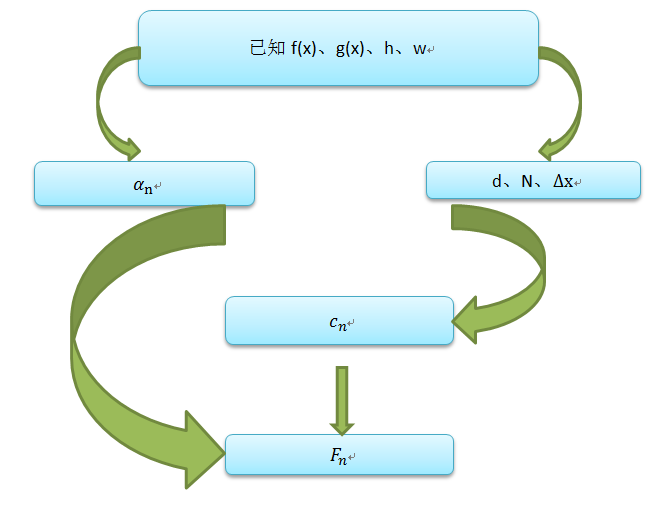
\includegraphics[width=.6\textwidth]{1.png}
\caption{问题三流程图}
\end{figure}

\section{绘制普通三线表格}
表格应具有三线表格式,因此常用 booktabs宏包,其标准格式如表~\ref{tab001}~所示。
\begin{table}[!htbp]
\caption{标准三线表格}\label{tab001} \centering
\begin{tabular}{ccccc}
\toprule[1.5pt]
$D$(in) & $P_u$(lbs) & $u_u$(in) & $\beta$ & $G_f$(psi.in)\\
\midrule[1pt]
 5 & 269.8 & 0.000674 & 1.79 & 0.04089\\
10 & 421.0 & 0.001035 & 3.59 & 0.04089\\
20 & 640.2 & 0.001565 & 7.18 & 0.04089\\
\bottomrule[1.5pt]
\end{tabular}
\end{table}

其绘制表格的代码及其说明如下。
\begin{tcode}
\begin{table}[!htbp]
\caption[标签名]{中文标题}
\begin{tabular}{cc...c}
\toprule[1.5pt]
表头第1个格   & 表头第2个格   & ... & 表头第n个格  \\
\midrule[1pt]
表中数据(1,1) & 表中数据(1,2) & ... & 表中数据(1,n)\\
表中数据(2,1) & 表中数据(2,2) & ... & 表中数据(2,n)\\
...................................................\\
表中数据(m,1) & 表中数据(m,2) & ... & 表中数据(m,n)\\
\bottomrule[1.5pt]
\end{tabular}
\end{table}
\end{tcode}

\bigskip
table环境是一个将表格嵌入文本的浮动环境。
tabular环境的必选参数由每列对应一个格式字符所组成:c表示居中,l表示左对齐,r表示右对齐,其总
个数应与表的列数相同。此外,\verb|@{文本}|可以出现在任意两个上述的列格式之间,其中的文本将被插入每一行
的同一位置。表格的各行以\verb|\\|分隔,同一行的各列则以\&分隔。
\verb|\toprule|、\verb|\midrule|和\verb|\bottomrule|三个命令是由booktabs宏包提供的,其
中\verb|\toprule|和\verb|\bottomrule|分别用来绘制表格的第一条(表格最顶部)和第三条(表格最底部)水平线,
\verb|\midrule|用来绘制第二条(表头之下)水平线,且第一条和第三条水平线的线宽为1.5pt,第二条水平线的线宽为1pt。
引用方法:“如表~\verb|\ref{标签名}|~所示”。


%参考文献
\begin{thebibliography}{9}%宽度9
 \bibitem{bib:one} ....
 \bibitem{bib:two} ....
\end{thebibliography}

\newpage
%附录
\begin{appendices}
\section{排队算法--matlab 源程序}
\begin{lstlisting}[language=matlab]
kk=2;[mdd,ndd]=size(dd);
while ~isempty(V)
[tmpd,j]=min(W(i,V));tmpj=V(j);
for k=2:ndd
[tmp1,jj]=min(dd(1,k)+W(dd(2,k),V));
tmp2=V(jj);tt(k-1,:)=[tmp1,tmp2,jj];
end
tmp=[tmpd,tmpj,j;tt];[tmp3,tmp4]=min(tmp(:,1));
if tmp3==tmpd, ss(1:2,kk)=[i;tmp(tmp4,2)];
else,tmp5=find(ss(:,tmp4)~=0);tmp6=length(tmp5);
if dd(2,tmp4)==ss(tmp6,tmp4)
ss(1:tmp6+1,kk)=[ss(tmp5,tmp4);tmp(tmp4,2)];
else, ss(1:3,kk)=[i;dd(2,tmp4);tmp(tmp4,2)];
end;end
dd=[dd,[tmp3;tmp(tmp4,2)]];V(tmp(tmp4,3))=[];
[mdd,ndd]=size(dd);kk=kk+1;
end; S=ss; D=dd(1,:);
 \end{lstlisting}
 \section{规划解决程序--lingo源代码}
\begin{lstlisting}[language=c]
kk=2;
[mdd,ndd]=size(dd);
while ~isempty(V)
    [tmpd,j]=min(W(i,V));tmpj=V(j);
for k=2:ndd
    [tmp1,jj]=min(dd(1,k)+W(dd(2,k),V));
    tmp2=V(jj);tt(k-1,:)=[tmp1,tmp2,jj];
end
    tmp=[tmpd,tmpj,j;tt];[tmp3,tmp4]=min(tmp(:,1));
if tmp3==tmpd, ss(1:2,kk)=[i;tmp(tmp4,2)];
else,tmp5=find(ss(:,tmp4)~=0);tmp6=length(tmp5);
if dd(2,tmp4)==ss(tmp6,tmp4)
    ss(1:tmp6+1,kk)=[ss(tmp5,tmp4);tmp(tmp4,2)];
else, ss(1:3,kk)=[i;dd(2,tmp4);tmp(tmp4,2)];
end;
end
    dd=[dd,[tmp3;tmp(tmp4,2)]];V(tmp(tmp4,3))=[];
    [mdd,ndd]=size(dd);
    kk=kk+1;
end;
S=ss;
D=dd(1,:);
 \end{lstlisting}
\end{appendices}

\end{document} 